
\section{M\'etodos}
Se descarg\'o la imagen de difusi\'on de un sujeto junto con su anat\'omica y una 
parcelaci\'on de esta. Los datos adquiridos en HCP ya estaban preprocesados
por lo que ning\'un tipo de preparaci\'on fue necesario. La parcelaci\'on 
fue utilizada para segmentar el cerebro en materia gris y blanca, as\'i como 
tambi\'en para generar una mascara del \'area de Broca. Dicho \'area  fue luego
mapeado sobre la materia blanca, consiguiendo as\'i un grupo de semillas.

\subsection{Tractogramas}
Dada una semilla y un mapa probabil\'istico de direcciones se denomina 
\textit{streamline} a uno de los posibles caminos que puede realizar una particula
comenzando desde la semilla. A su vez, dada una cantidad f\'inita de 
part\'iculas, se llama tractograma a la matriz que muestra la proporci\'on de
part\'iculas que pas\'o por cada voxel una vez finalizado el algoritmo. Luego 
todos los valores dentro de los tractogramas fueron escalados utilizando la 
funci\'on logaritmo, y normalizados entre 0 y 1, donde 1 representa que todas
las \textit{streamlines} pasaron por ese voxel. 

Dipy es una librer\'ia para python que contiene, 
entre otras herramientas, varios algor\'itmos para generar \textit{streamlines}.
Para este trabajo eleg\'imos utilizar la implementaci\'on de
\textit{LocalTracking} (LT de aqu\'i en mas) que se encuentra en el paquete
dipy.tracking.local; y una funci\'on pr\'opia (MSL de aqu\'i
en mas) que utiliza la clase \textit{ProbabilisticDirectionGetter} de
dipy.direction y la funci\'on \textit{markov\_streamlines} de dipy.tracking.markov.

Es importante destacar que como la interfaz del \textit{DirectionGetter} (DG) 
no es compatible con la funci\'on \textit{markov\_streamlines} (ver documentaci\'on
de dipy) fue necesario crear una clase que hiciera de puente entre ambas. Dicha 
clase se encuentra en el paquete scripts.proba, y lo que hace es seleccionar 
una direcci\'on inicial al azar entre las propuestas por DG, y la direcci\'on
propuesta por DG luego de cada paso hasta que se sale de la mascara de materia
blanca. 

Para utilizar cada uno de estos algoritmos es necesario encuadrar la informaci\'on
de dMRI dentro de un modelo. En este caso se utiliz\'o el modelo 
\textit{ Constrained Spherical Deconvolve Model} para ambos.  
Por cuestiones de \textit{performance} se gener\'o un script para computar en
paralelo los \textit{streamlines} de cada semilla por cada algoritmo. Dicho script 
fue ejecutado en el cluster del INRIA.

\textbf{notebook: Tractograf\'ia probabil\'istica.}

\subsection{Estabilidad Algoritmos}

Para determinar si el tractograma medio converg\'ia se utiliz\'o un n\'umero 
peque\~no de semillas y la t\'ecnica  estad\'istica de \textit{bootstrap}.
En principio se comput\'o un total de 15.000 \textit{streamlines} por semilla.
Luego por cada semilla se calcul\'o el tractograma medio y la varianza de 
cada voxel utilizando mil submuestras aleator\'ias del mismo tama\~o. Esto se
repitio\'o con varios tama\~nos de submuestra para ver as\'i que tan variable
era la muestra a medida que crec\'ia.

\subsection{Hierarchical Clustering}

Finalmente se utiliza la implementaci\'on de \textit{Hirarchical Clustering} 
que se encuentra en el paquete scipy.cluster.hierarchy, utilizando la distancia
euclidea entre ellos. El resultado de aplicar este algoritmo se puede representar
en un dendograma. La librer\'ia tambi\'en presenta distintos m\'etodos para 
cortar dividir dicha representaci\'on en varios clusters. 

Una vez obtenida la parcelaci\'on de las semillas es necesario mapear la misma
sobre la materia gris, dado que recordemos que las semillas se encuentran 
en medio de ambas. Para esto utilizamos dos m\'etodos distintos, el primero 
consiste simplemente en dilatar las parcelas por turnos hasta que las mismas se
encuentran con la materia gris, en orden de tama\~no decreciente. El hecho de
hacerlo por turnos permite que las parcelas de menor tama\~no no sean absorbidas
por las de mayor. El segundo m\'etodo consiste en utilizar el algoritmo de 
\textit{Fast Marching Method} para definir la distancia desde las semillas hasta
la materia gris, y luego recorrer el campo gradiente de las distancias partiendo
desde cada semilla.

\section{Resultados}

\subsection{Tractogramas}

Sobre un total de 2600 semillas, los algoritmos MSL y LT presentaron resultados
visualmente similares en la mayor parte de los casos, aunque MSL siempre
gener\'o \textit{Streamlines} mas cortos; en algunos casos incluso nulo. 
Las Figuras \ref{fig:msl99} y \ref{fig:lt99} muestra los resultados de ambos 
algoritmos para una misma semilla. Idem Figuras \ref{fig:msl107} y \ref{fig:lt107}.

\begin{figure}[h!]
   \centering
    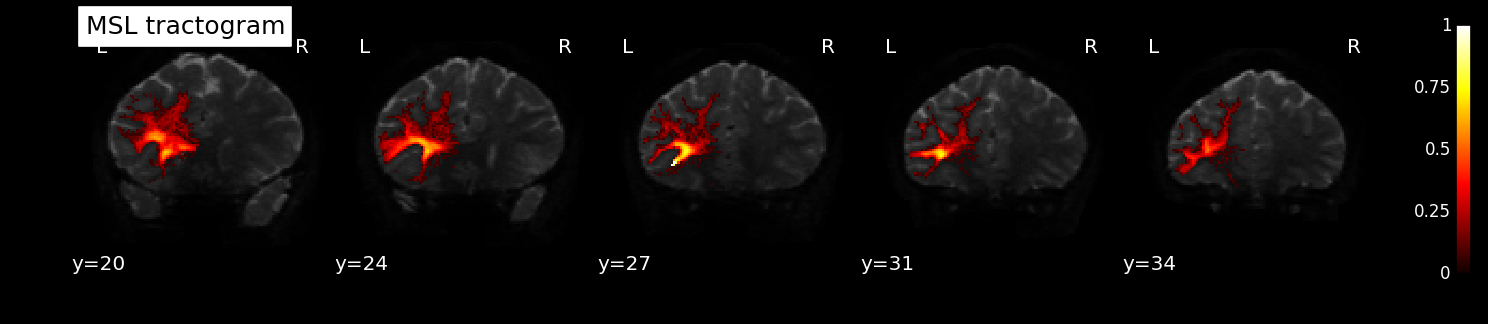
\includegraphics[width=\textwidth]{img/msl_99_123_54.png}
    \caption{Resultado para algoritmo MSL}
    \label{fig:msl99}
\end{figure}

\begin{figure}[h!]
   \centering
    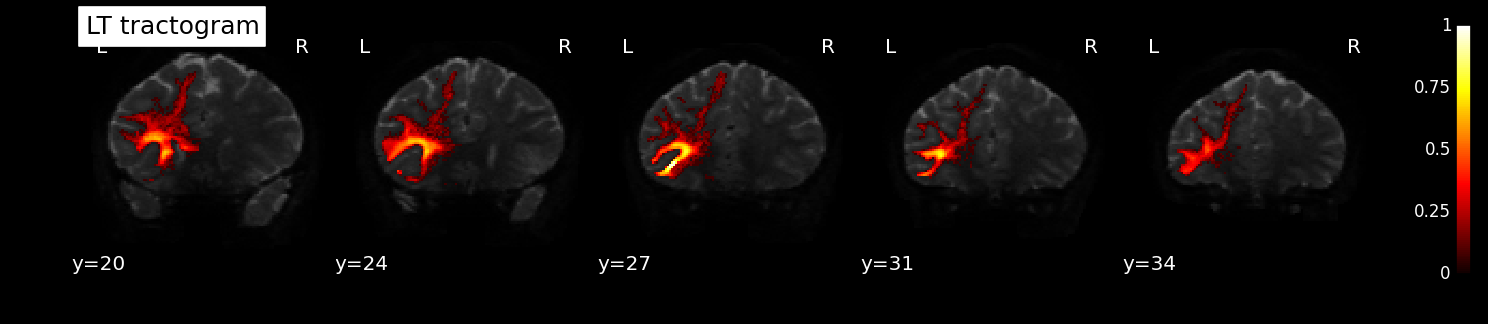
\includegraphics[width=\textwidth]{img/lt_99_123_54.png}
    \caption{Resultado para algoritmo LT}
    \label{fig:lt99}
\end{figure}

\begin{figure}[h!]
   \centering
    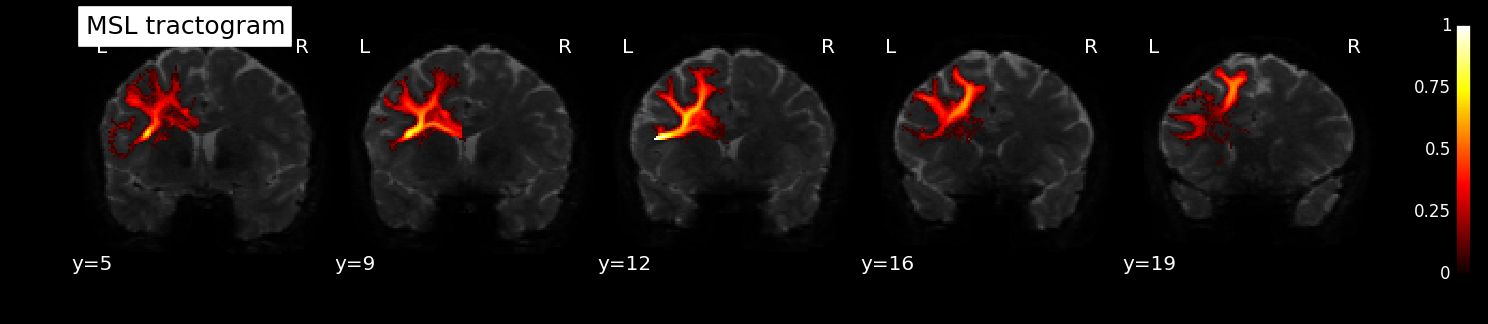
\includegraphics[width=\textwidth]{img/msl_107_111_66.png}
    \caption{Resultado para algoritmo MSL}
    \label{fig:msl107}
\end{figure}

\begin{figure}[h!]
   \centering
    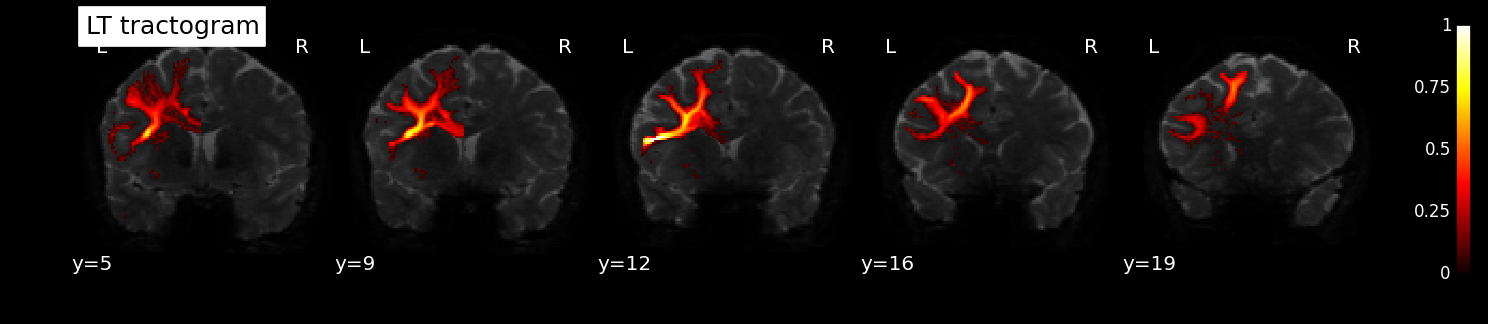
\includegraphics[width=\textwidth]{img/lt_107_111_66.png}
    \caption{Resultado para algoritmo LT}
    \label{fig:lt107}
\end{figure}

\subsection{Convergencia Algor\'itmica}
Las Figuras \ref{fig:mmean}; \ref{fig:mstd1} y \ref{fig:mstd2} muestran el valor
de la media y el desvio estandar para todos los voxels pertenecientes al tractograma
de una semilla creado con el algor\'itmo MSL. Se puede ver claramente que el 
algoritmo converge. Las Figuras \ref{fig:lmean}; \ref{fig:lstd1} y \ref{fig:lstd2} 
muestran lo mismo para el algoritmo LT.

\begin{figure}[h!]
   \centering
    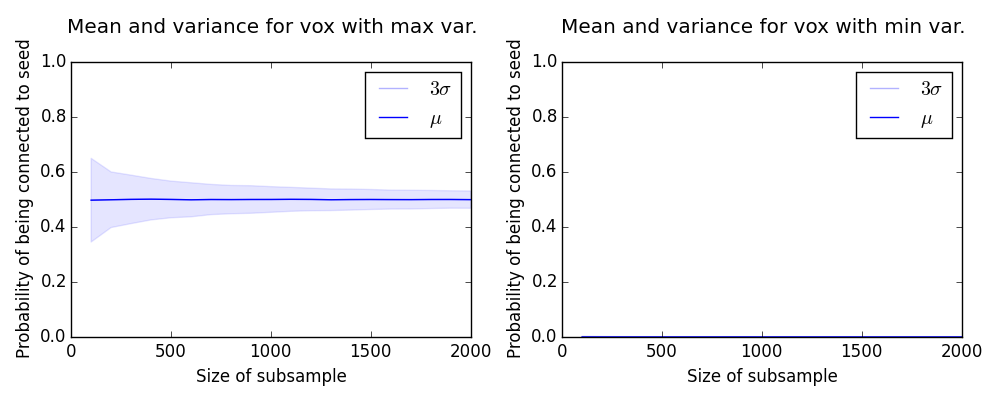
\includegraphics[width=\textwidth]{img/mvmsl_97_124_62.png}
    \caption{Resultado para algoritmo MSL}
    \label{fig:mm94}
\end{figure}

\begin{figure}[h!]
   \centering
    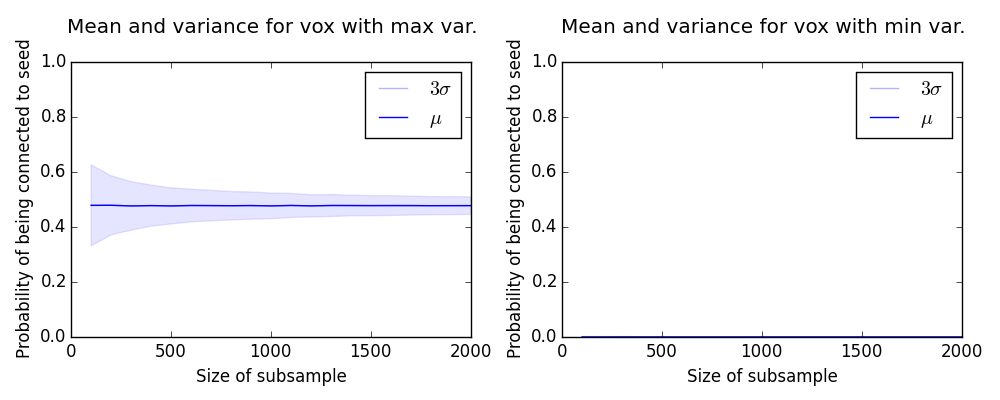
\includegraphics[width=\textwidth]{img/mvlt_97_124_62.png}
    \caption{Resultado para algoritmo LT}
    \label{fig:ml94}
\end{figure}

Las Figuras \ref{fig:mm99} y \ref{fig:ml94} corresponden a los resultados obtenidos
en los voxels que pose\'ian mayor y menor desvio estandar para los algoritmos 
MSL y LT respectivamente. 
Se puede ver que los voxels de mayor desvio convergen a medida que la poblaci\'on 
crece. El voxel de menor desvio probablemente est\'e compuesto por poblaciones donde solo un 
\textit{streamline} lo cruz\'o, por eso la media es casi nula y no var\'ia.

\begin{figure}[h!]
   \centering
    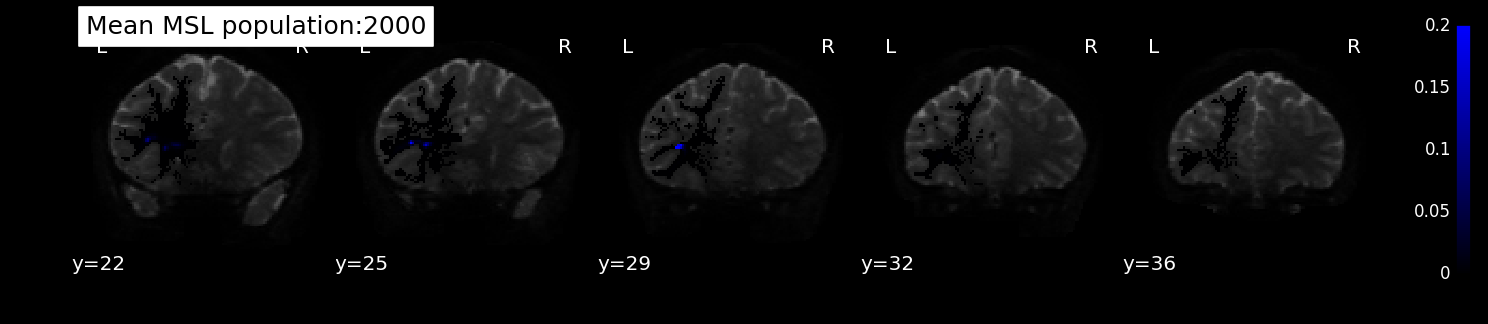
\includegraphics[width=\textwidth]{img/msl_all_mean.png}
    \caption{Media para MSL utilizando 2000 semillas}
    \label{fig:mmean}
\end{figure}

\begin{figure}[h!]
   \centering
    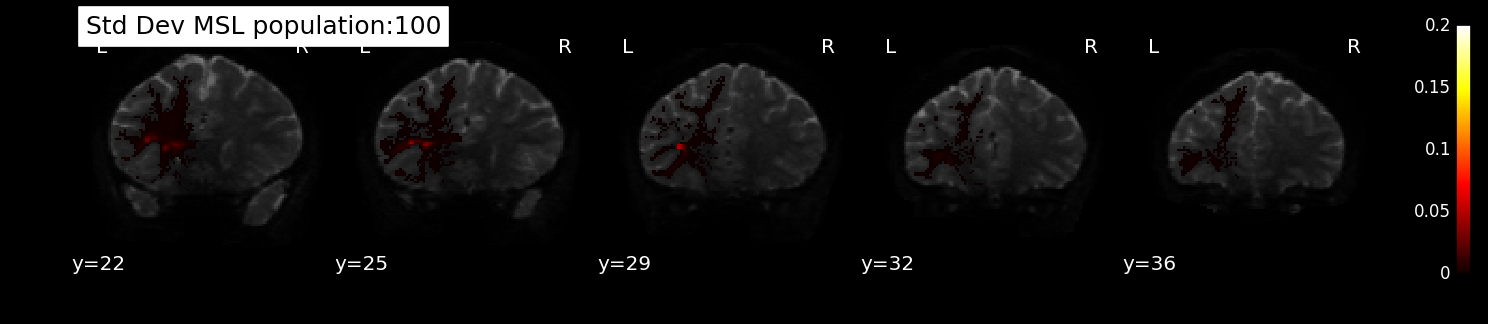
\includegraphics[width=\textwidth]{img/msl_allstd1.png}
    \caption{Desvio Estandar MSL utilizando 100 semillas}
    \label{fig:mstd1}
\end{figure}

\begin{figure}[h!]
   \centering
    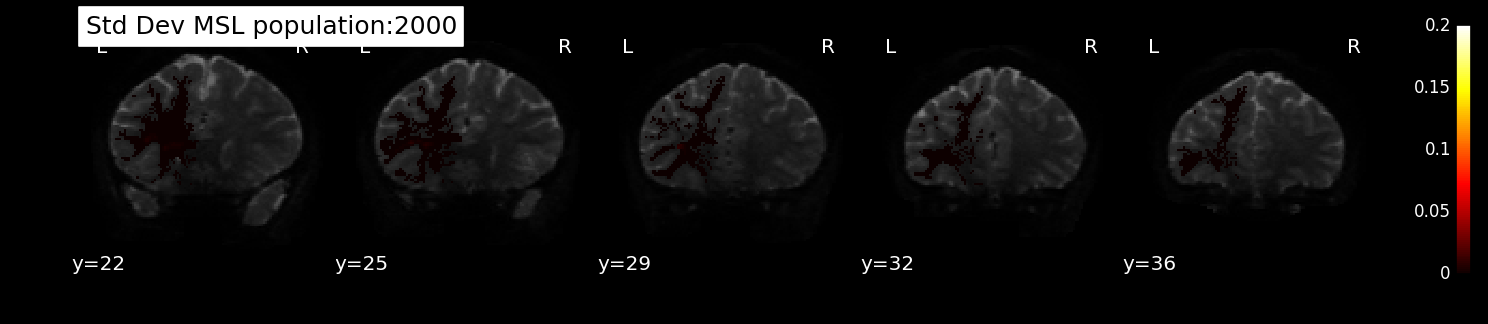
\includegraphics[width=\textwidth]{img/msl_allstd2.png}
    \caption{Desvio Estandar MSL utilizando 2000 semillas}
    \label{fig:mstd2}
\end{figure}

\begin{figure}[h!]
   \centering
    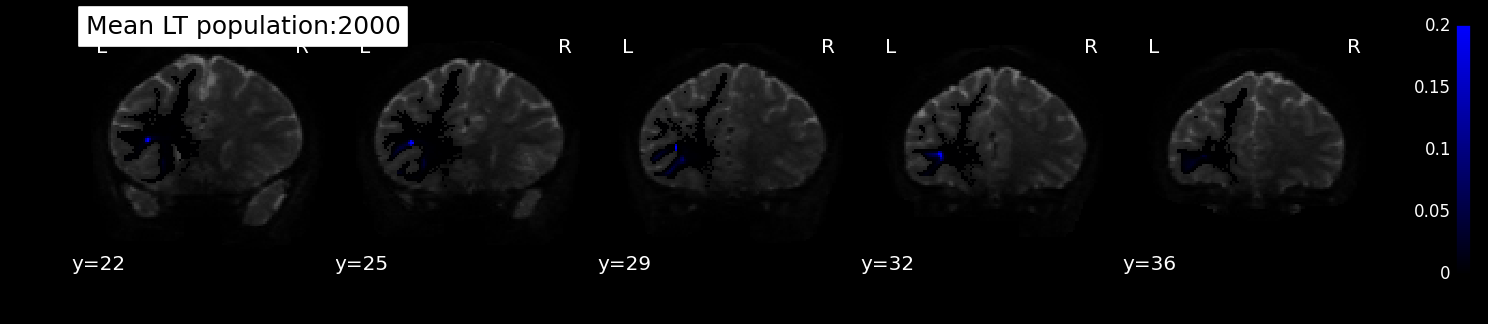
\includegraphics[width=\textwidth]{img/lt_all_mean.png}
    \caption{Media para LT utilizando 2000 semillas}
    \label{fig:lmean}
\end{figure}

\begin{figure}[h!]
   \centering
    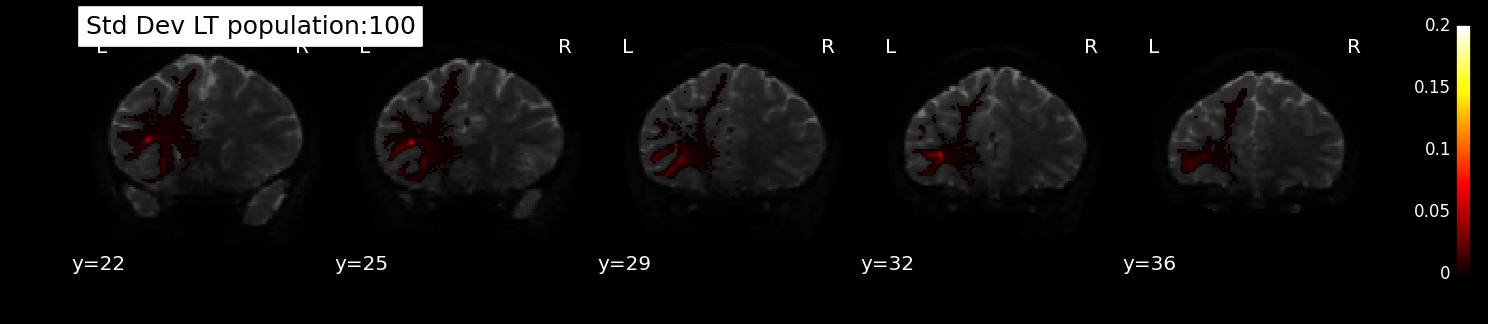
\includegraphics[width=\textwidth]{img/lt_allstd1.png}
    \caption{Desvio Estandar para LT utilizando 100 semillas}
    \label{fig:lstd1}
\end{figure}

\begin{figure}[h!]
   \centering
    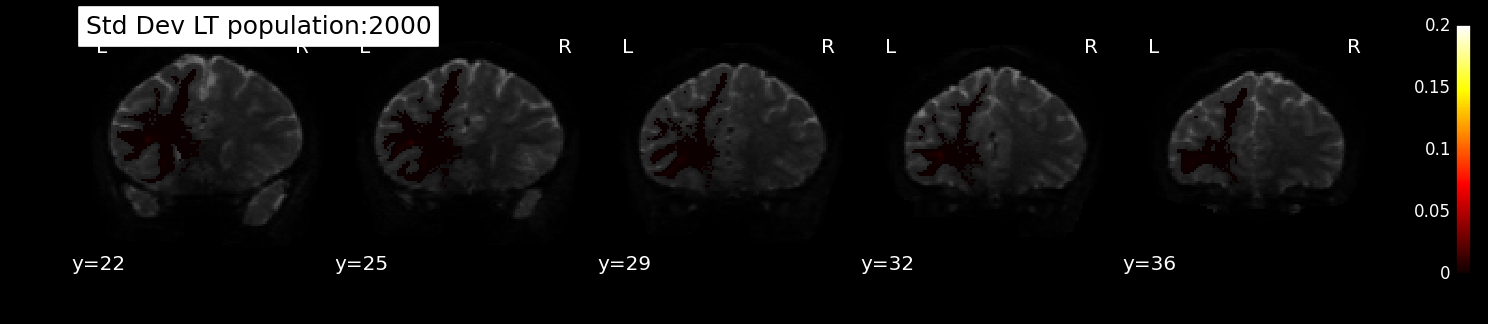
\includegraphics[width=\textwidth]{img/lt_allstd2.png}
    \caption{Desvio Estandar para LT utilizando 2000 semillas}
    \label{fig:lstd2}
\end{figure}

\subsection{Agglomerative Hierarchical Clustering}

Las Figuras \ref{fig:dendo1} y \ref{fig:dendo2} muestran el dendograma generado
en distintos niveles de profundidad. Las Figuras \ref{fig:infla} y \ref{fig:rec}
muestran el resultado de dividir el \'area de broca en 4 parcelaciones distintas
utilizando los m\'etodos de dilataci\'on y gradiente respectivamente. La Figura
\ref{infvsrec} muestra una comparaci\'on mas fina entre los resultados.  
Dos de las parcelas se pueden distinguir facilmente, mientras que las restantes
est\'an definidas por no mas de 10 voxels. - si mal no recuerdo estas parcelas
sobreviven a mas divisiones, probar -. 

Tambi\'en es importante notar que el m\'etodo de dilataci\'on mapea parcelas
fuera del \'area de broca, aunque esto era esperable.

\begin{figure}[h!]
   \centering
    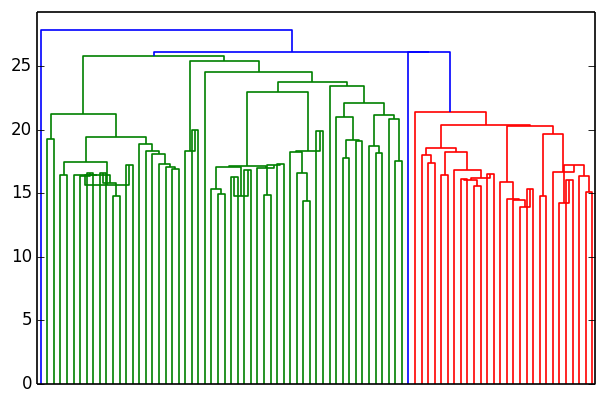
\includegraphics[width=\textwidth]{img/dendo1.png}
    \caption{Dendograma de 15 niveles}
    \label{fig:infla}
\end{figure}

\begin{figure}[h!]
   \centering
    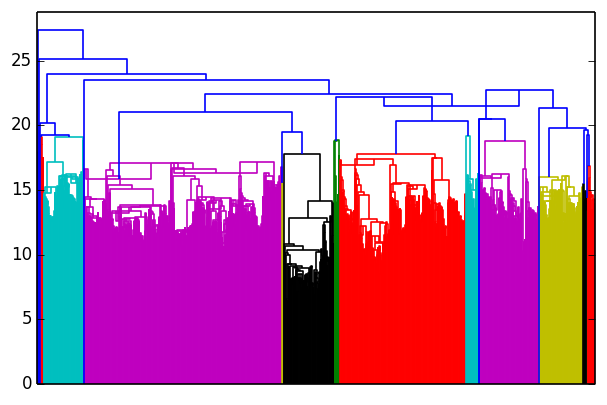
\includegraphics[width=\textwidth]{img/dendo2.png}
    \caption{Dendograma de 30 niveles}
    \label{fig:infla}
\end{figure}

\begin{figure}[h!]
   \centering
    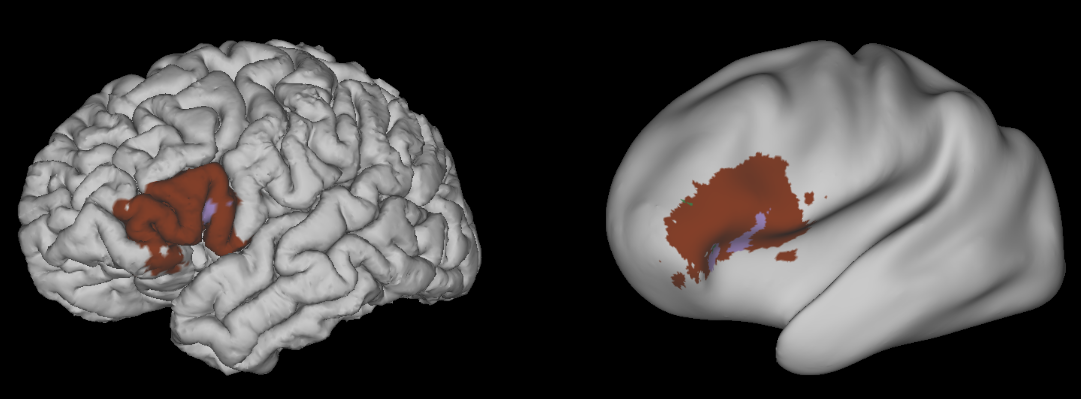
\includegraphics[width=\textwidth]{img/inflated.png}
    \caption{Mapeo obtenido utilizando dilataci\'on para cuatro parcelas}
    \label{fig:infla}
\end{figure}

\begin{figure}[h!]
   \centering
    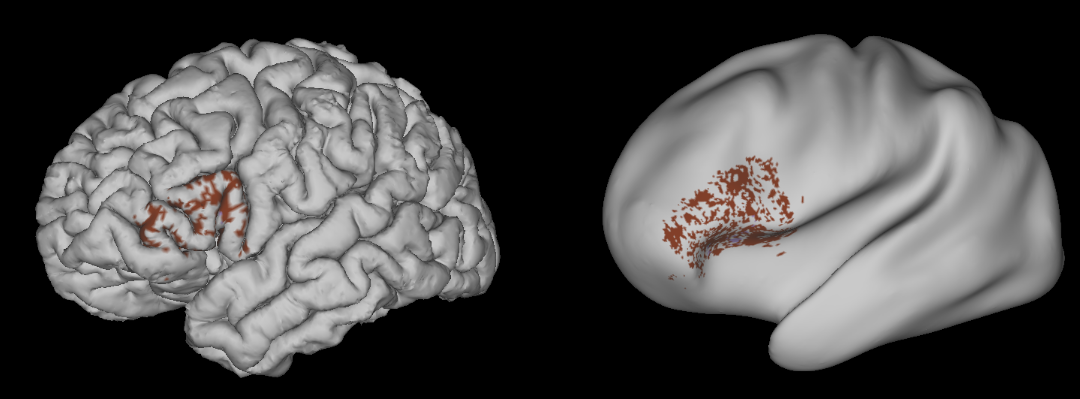
\includegraphics[width=\textwidth]{img/reconstructed.png}
    \caption{Mapeo obtenido utilizando el campo gradiente para cuatro parcelas}
    \label{fig:rec}
\end{figure}

\begin{figure}[h!]
   \centering
    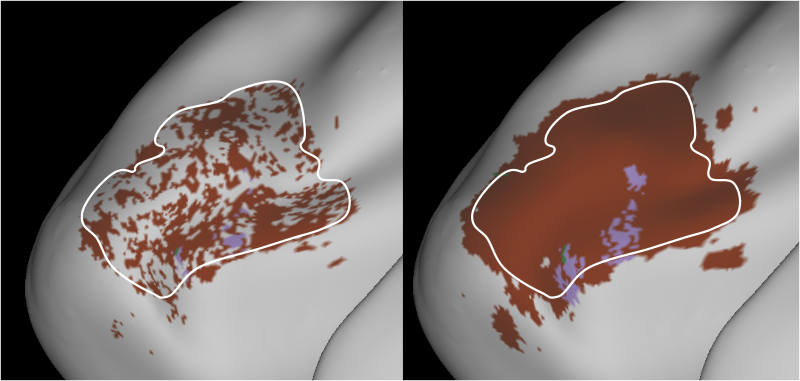
\includegraphics[width=\textwidth]{img/inf_vs_rec.png}
    \caption{Acercamiento a la parcelaci\'on obtenida junto con los l\'imites
            del \'area de Broca}
    \label{fig:infvsrec}
\end{figure}
